Ein Körper bewegt sich auf einer geraden Linie. Das Diagramm zeigt seine Geschwindigkeit.
\begin{center}
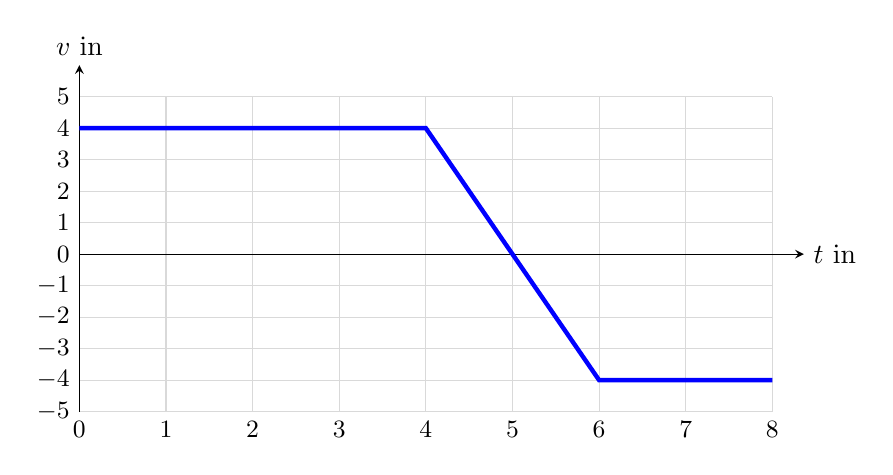
\begin{tikzpicture}[>=stealth, x=1.1cm, y=0.4cm]
 \draw[gray!30] (0,-5) grid[xstep=1, ystep=1] (8,5);
 \draw[->] (0,0) -- (8.364,0) node[right] {$t$ in \si{\second}};
 \draw[->] (0,-5) -- (0,6) node[above] {$v$ in \si{\meter\per\second}};
 \foreach \tk in {0,1,2,3,4,5,6,7,8} \node[below] at (\tk,-5) {\small $\tk$};
 \foreach \yk in {-5,-4,-3,-2,-1,0,1,2,3,4,5} \node[left] at (0,\yk) {\small $\yk$};
 \draw[ultra thick, blue] (0,4) -- (4,4) -- (6,-4) -- (8,-4);
\end{tikzpicture}
\end{center}
\begin{abcliste}
\abc Bestimmen Sie die mittlere Geschwindigkeit von \SI{0}{\second} bis \tEO.
\abc Drei Antworten aus der Klasse lauten:
\begin{itemize}
\item[(i)] „$\bar v = \SI{4}{\meter\per\second}$, der Körper ist ja fast immer mit \SI{4}{\meter\per\second} unterwegs.“
\item[(ii)] „$\bar v = \SI{8}{\meter}$, das ist die Fläche unter dem Graphen.“
\item[(iii)] „$\bar v = 0$, das Mittel aus der Anfangs- und der Endgeschwindigkeit.“
\end{itemize}
Was ist an jeder dieser Antworten falsch?
\end{abcliste}
